% $File: main.tex
% $Date: Thu May 21 22:05:07 2015 +0800
% $Author: jiakai <jia.kai66@gmail.com>

\documentclass[bachelor]{thuthesis}
%\documentclass[master]{thuthesis}
%\documentclass[doctor]{thuthesis}
% \documentclass[%
%   bachelor|master|doctor|postdoctor, % mandatory option
%   secret,
%   openany|openright,
%   arialtoc,arialtitle]{thuthesis}

% 所有其它可能用到的包都统一放到这里了,可以根据自己的实际添加或者删除。
\usepackage{thutils}
\usepackage{pdfpages}

% 你可以在这里修改配置文件中的定义,导言区可以使用中文。
\def\myname{贾开}

\begin{document}


%%% 封面部分
\frontmatter

%%% Local Variables:
%%% mode: latex
%%% TeX-master: t
%%% End:
\secretlevel{绝密} \secretyear{2100}

\ctitle{基于非监督深度学习的医学影像特征提取研究}
% 根据自己的情况选,不用这样复杂
\makeatletter
\ifthu@bachelor\relax\else
  \ifthu@doctor
    \cdegree{工学博士}
  \else
    \ifthu@master
      \cdegree{工学硕士}
    \fi
  \fi
\fi
\makeatother


\cdepartment[计算机]{计算机科学与技术系}
\cmajor{计算机科学与技术}
\cauthor{贾开}
\csupervisor{宋亦旭~~副研究员}
% 如果没有副指导老师或者联合指导老师,把下面两行相应的删除即可。
%\cassosupervisor{陈文光教授}
%\ccosupervisor{某某某教授}
% 日期自动生成,如果你要自己写就改这个cdate
%\cdate{\CJKdigits{\the\year}年\CJKnumber{\the\month}月}

% 博士后部分
% \cfirstdiscipline{计算机科学与技术}
% \cseconddiscipline{系统结构}
% \postdoctordate{2009年7月——2011年7月}

\etitle{Research on Unsupervised Deep Feature Learning on Medical Images}
% 这块比较复杂,需要分情况讨论:
% 1. 学术型硕士
%    \edegree:必须为Master of Arts或Master of Science(注意大小写)
%              “哲学、文学、历史学、法学、教育学、艺术学门类,公共管理学科
%               填写Master of Arts,其它填写Master of Science”
%    \emajor:“获得一级学科授权的学科填写一级学科名称,其它填写二级学科名称”
% 2. 专业型硕士
%    \edegree:“填写专业学位英文名称全称”
%    \emajor:“工程硕士填写工程领域,其它专业学位不填写此项”
% 3. 学术型博士
%    \edegree:Doctor of Philosophy(注意大小写)
%    \emajor:“获得一级学科授权的学科填写一级学科名称,其它填写二级学科名称”
% 4. 专业型博士
%    \edegree:“填写专业学位英文名称全称”
%    \emajor:不填写此项
\edegree{Doctor of Engineering}
\emajor{Computer Science and Technology}
\eauthor{Kai Jia}
\esupervisor{Yixu Song}
%\eassosupervisor{Chen Wenguang}
% 这个日期也会自动生成,你要改么?
% \edate{December, 2005}

% 定义中英文摘要和关键字
\begin{cabstract}
    如何提取出兼具鲁棒性和区分性的特征是医学影像处理中的一个重要问题。
许多传统方法基于人工设计的浅层特征,无法在一般任务中达到足够的性能;
基于监督学习的方法依赖于对匹配点的人工标注;
而大部分非监督学习的方法又没有显式对特征应具有的不变性进行描述,
其性能没有根本保障。为了解决以上问题,
在本文中我们基于非监督学习的框架,
在深度卷积神经网络的损失函数里显式加入对特征鲁棒性和区分性的要求,
从而得到更好的特征提取器。同时我们提出了新的特征评测标准,
能在不通过其它图像处理任务来间接反映特征性能、
也不需要人工标注对应点的情况下,简明直接地完成对特征本身性能的评价。
实验结果证明我们的特征提取器优于之前的层叠卷积ISA,
这有望进一步提升许多医学影像处理算法的性能。

\end{cabstract}

\ckeywords{深度学习, 非监督学习, 特征提取, 医学影像处理, 卷积神经网络}

\begin{eabstract}
    hello, world
\end{eabstract}

\ekeywords{deep learning, unsupervised learning, liver image segmentation}

% 设置 PDF 文档的作者、主题等属性
\makeatletter
\thu@setup@pdfinfo
\makeatother
\makecover

% 目录
\tableofcontents


%%% 正文部分
\mainmatter
% $File: chap01.tex
% $Date: Thu May 21 21:42:49 2015 +0800
% $Author: jiakai <jia.kai66@gmail.com>

\chapter{引言}
本章主要阐述本文要研究的问题,其研究背景及研究现状,
指出问题本身在学术及应用上的价值和难点,引出后续工作。

\section{非监督深度特征学习}
简述深度学习、非监督学习、特征提取等

\section{医学影像处理}
医学影像的特点、研究的意义、难点,深度学习与此的结合。

并简述肝脏分割的现有方法,引出本文以刚脏分割作为 example task。

% vim: filetype=tex foldmethod=marker foldmarker=f{{{,f}}}

% $File: chap02.tex
% $Date: Thu May 21 22:10:39 2015 +0800
% $Author: jiakai <jia.kai66@gmail.com>

\chapter{模型选取与训练方法}


\section{源于统计的ISA模型}

\subsection{从PCA到ISA}

\subsection{对ISA的三种解读}

\subsection{层叠卷积ISA}


\section{深度卷积神经网络}

\subsection{动机}
指出纯统计方法缺乏先验,并提出需要把非监督学习转换成监督学习并以引入先验知识。

\subsection{基本组成元素}

\subsection{目标函数}
\subsubsection{分类输出:Softmax与交叉熵损失函数}
\subsubsection{直接特征输出:度量学习}


\section{训练方法}

\subsection{数值优化方法}

\subsubsection{梯度下降}
\subsubsection{随机梯度下降}

\subsection{数据增广}
简要形式化描述希望特征对变换$F(A, \gamma)=(affine(A), gamma(\gamma))$
满足的不变性

\subsubsection{Gamma变换}

\subsubsection{三维仿射变换的表示、分解与采样}

% vim: filetype=tex foldmethod=marker foldmarker=f{{{,f}}}


% $File: chap03.tex
% $Date: Thu May 21 22:03:43 2015 +0800
% $Author: jiakai <jia.kai66@gmail.com>

\chapter{实验与结果}

\section{实验细节}

\subsection{实验环境及代码实现概述}

\subsection{模型参数设定}

\subsection{训练数据}


\section{评测方法}

score = AUC + sparseness

\subsection{单点匹配的判定}
带符号边界距离,GPU KNN计算,cos/L2 dist

\subsection{ROC曲线及曲线下面积}

\subsection{稀疏程度的衡量}


\section{实验结果}
曲线,表格


% vim: filetype=tex foldmethod=marker foldmarker=f{{{,f}}}



% $File: chap04.tex
% $Date: Thu May 21 22:04:15 2015 +0800
% $Author: jiakai <jia.kai66@gmail.com>

\chapter{讨论}

总结,贡献,不足,future work

% vim: filetype=tex foldmethod=marker foldmarker=f{{{,f}}}






%%% 其它部分
\backmatter

% 本科生要这几个索引,研究生不要。选择性留下。
\makeatletter
\ifthu@bachelor
  % 插图索引
  \listoffigures
  % 表格索引
  \listoftables
  % 公式索引
  %\listofequations
\fi
\makeatother


% 参考文献
% 注意至少需要引用一篇参考文献,否则下面两行可能引起编译错误。
% 如果不需要参考文献,请将下面两行删除或注释掉。
\bibliographystyle{thubib}
\bibliography{refs}


% 致谢
%%% Local Variables:
%%% mode: latex
%%% TeX-master: "../main"
%%% End:

\begin{ack}
  衷心感谢导师 xxx 教授和物理系 xxx 副教授对本人的精心指导。他们的言传身教将使
  我终生受益。

  在美国麻省理工学院化学系进行九个月的合作研究期间,承蒙 xxx 教授热心指导与帮助,不
  胜感激。感谢 xx 实验室主任 xx 教授,以及实验室全体老师和同学们的热情帮助和支
  持!本课题承蒙国家自然科学基金资助,特此致谢。

  感谢 \thuthesis,它的存在让我的论文写作轻松自在了许多,让我的论文格式规整漂亮了
  许多。
\end{ack}


% 附录
\begin{appendix}
% $File: appendix01.tex
% $Date: Sun May 17 20:03:45 2015 +0800
% $Author: jiakai <jia.kai66@gmail.com>

\chapter{外文资料原文}
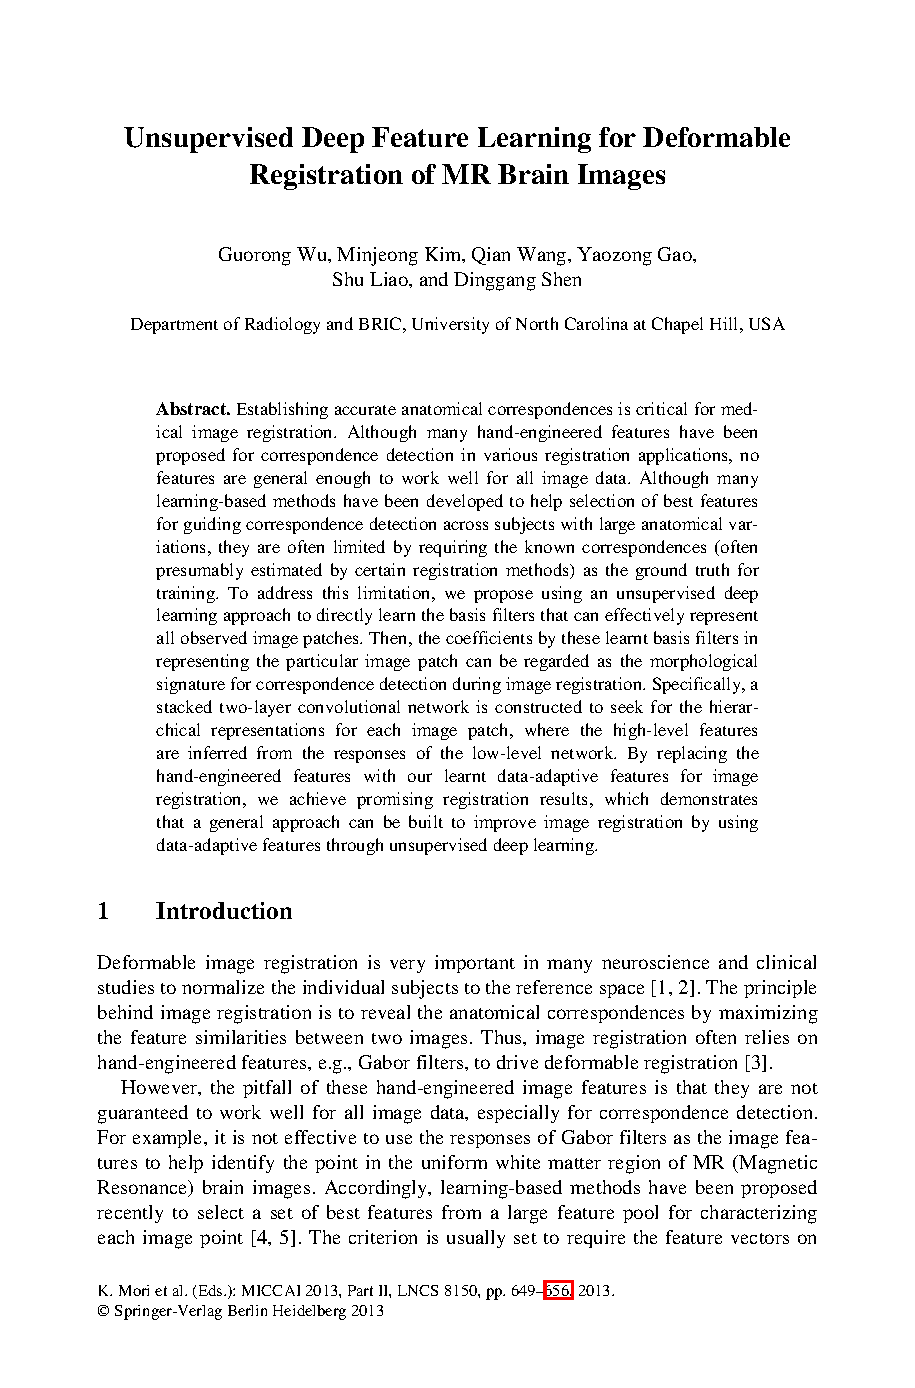
\includepdf[pages={-},scale=.9,pagecommand={}]{res/trans-english.pdf}

\chapter{外文资料的书面翻译}
最后再写吧


% vim: filetype=tex foldmethod=marker foldmarker=f{{{,f}}}

\end{appendix}

% 个人简历
%\include{data/resume}

\end{document}

% vim: filetype=tex foldmethod=marker foldmarker=f{{{,f}}}
